
\chapter{Greffon Statique-Dynamique (StaDy)}
\label{sec:stady}

\chapterintro


Dans ce chapitre nous présentons l'architecture générale du greffon \stady,
notre implémentation de la méthode présentée aux chapitres~\ref{sec:ncd},
\ref{sec:swd} et~\ref{sec:method}, ainsi que certains détails d'implémentation
en partie~\ref{sec:stady-implem}.
En partie~\ref{sec:stady-exp} nous présentons les résultats de nos
expérimentations visant à mesurer la capacité de diagnostic des échecs de preuve
et les performances de \stady.


\section{Implémentation du greffon \stady}
\label{sec:stady-implem}


%\begin{landscape}
\begin{center}
  \begin{figure}[tb]
    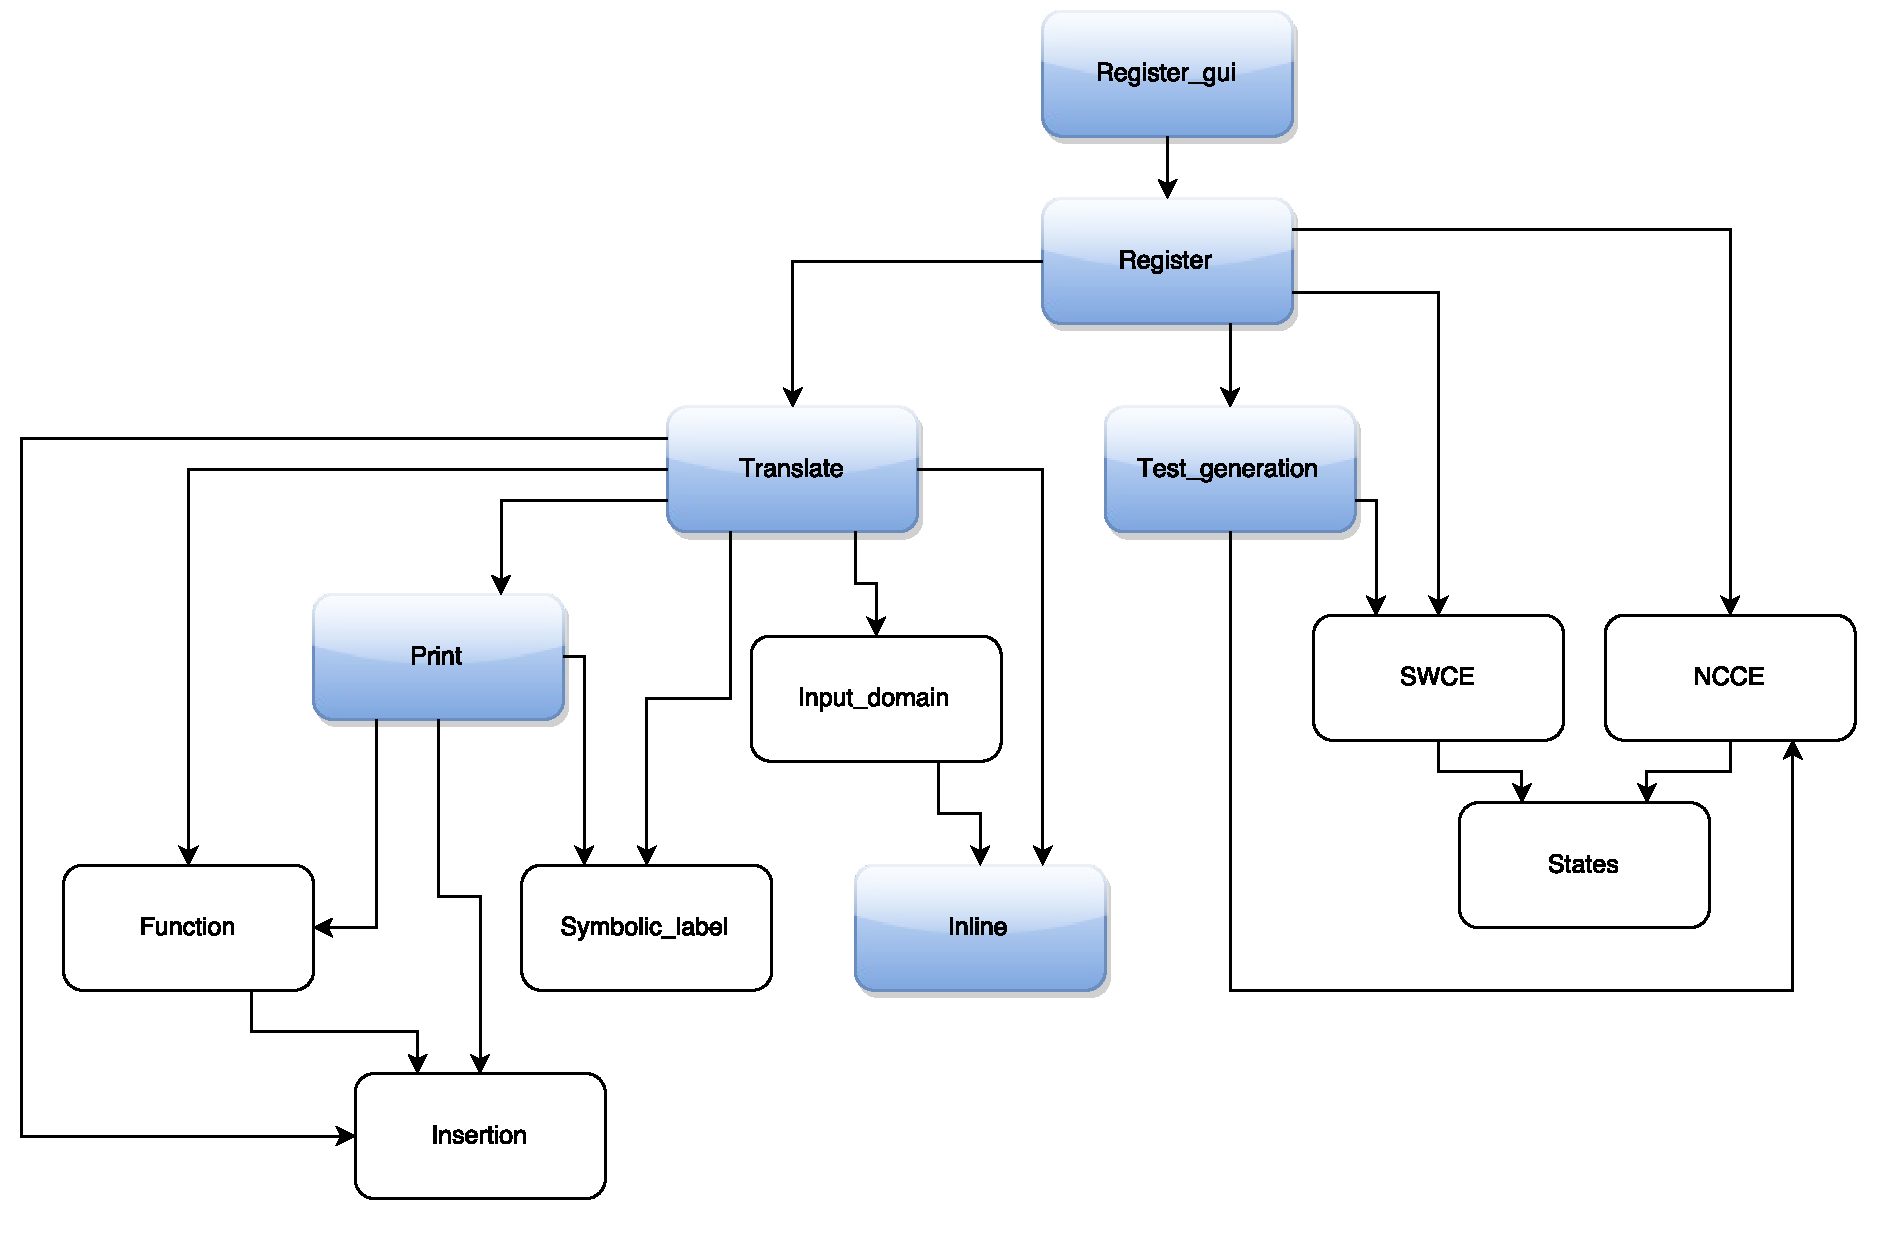
\includegraphics[scale=.5]{figures/stady_architecture.pdf}
    \vspace{-11cm}
    \caption{Architecture de \textsc{StaDy}
      \label{fig:stady-architecture}}
  \end{figure}
\end{center}
%\end{landscape}


\begin{figure}[tb]\scriptsize
  \begin{center}
    \begin{tabular}{lrr}
      \hline
      Module & Lignes de code & Lignes de commentaires \\
      \hline
      \textsc{Function} & 33 & 0 (0\%)\\
      \textsc{Inline} & 168 & 19 (10\%)\\
      \textsc{Input\_domain} & 430 & 6 (1\%)\\
      \textsc{Insertion} & 55 & 0 (0\%)\\
      \textsc{NCCE} & 55 & 0 (0\%)\\
      \textsc{Print} & 108 & 3 (2\%)\\
      \textsc{Register\_gui} & 83 & 0 (0\%)\\
      \textsc{Register} & 186 & 1 (0\%)\\
      \textsc{States} & 76 & 6 (7\%)\\
      \textsc{SWCE} & 64 & 0 (0\%)\\
      \textsc{Symbolic\_label} & 21 & 0 (0\%)\\
      \textsc{Test\_generation} & 147 & 8 (5\%)\\
      \textsc{Translate} & 1413 & 20 (1\%)\\
      Autres & 827 & 58 (7\%)\\
      \textbf{Total} & 3236 & 115 (3\%)\\ \hline
    \end{tabular}
  \end{center}
  \vspace{-3mm}
  \caption{Lignes de code et de commentaires par module}    
  \label{fig:stady-wc}
\end{figure}


La figure~\ref{fig:stady-architecture} présente l'architecture de \stady, elle
offre une vue simplifiée des relations entre les différents modules OCaml (nous
ferons l'amalgame entre les modules et les fichiers) qui composent l'outil.
Chaque bloc représente un module et la relation $A \rightarrow B$ symbolise le
fait que $A$ fait appel à $B$.
Les blocs dont le fond est blanc représentent des modules décrivant un ou
plusieurs types de données et implémentant les opérations sur ce(s) type(s).
Les blocs dont le fond est coloré représentent des modules implémentant une
fonctionnalité importante de l'outil.

La figure~\ref{fig:stady-wc} détaille le nombre de lignes de code et de
commentaires (en ne comptant pas les lignes vides) de l'implémentation de
\stady.
Au total, \stady compte un peu plus de 3200 lignes de code OCaml, ce qui
correspond à un greffon de \framac de taille moyenne.
En effet, le greffon \eacsltoc, de complexité similaire, compte environ 4200
lignes de code OCaml, ce qui reste loin derrière les greffons les plus
importants et complexes de \framac, \Value et \Wp, qui comptent chacun environ
30000 lignes de code OCaml.

Le module \textsc{Register} pilote les autres modules de \stady, tandis que le
module \textsc{Register\_gui} implémente les comportements souhaités du greffon
dans l'interface graphique de \framac.
Les deux fonctionnalités centrales de l'outil sont, conformément à ce qui est
décrit dans le chapitre~\ref{sec:traduction}, la traduction des annotations,
effectuée par le module \textsc{Translate}, et la génération de tests, pilotée
par le module \textsc{Test\_generation}.
Donnons maintenant une vue d'ensemble de ces opérations et des modules qui les
composent.


\subsection{Traduction des annotations}


Afin de traduire les annotations \eacsl en C nous avons besoin de définir des
types de données spécifiques.
Le module \textsc{Insertion} définit le type des insertions de code telles
qu'elles sont définies au chapitre~\ref{sec:traduction}.
Le module \textsc{Symbolic\_label} définit les labels symboliques qui permettent
d'associer un endroit du programme aux insertions de code (début ou fin d'une
fonction, début ou fin d'une boucle, avant ou après une instruction).
Le module \textsc{Function} définit le type de données des fonctions générées
de toute pièce par la traduction.
Le module \textsc{Input\_domain} définit des types de données représentant les
domaines et les différentes contraintes sur les variables en entrées du
programme (c'est-à-dire les variables en entrée de la fonction sous vérification
et les variables globales).

Les types définis par \textsc{Function} et \textsc{Insertion} sont des
extensions des types de l'arbre de syntaxe abstraite fournis par \framac, ils
nous permettent de ne pas modifier l'arbre de syntaxe abstraite du programme et
de stocker les insertions de code en de hors de l'arbre.
En effet, la modification de l'arbre de syntaxe abstraite par les greffons de
\framac est une opération complexe car il faut maintenir les relations
des données entre l'état {\em avant} et {\em après} la modification, ce qui est
source d'erreurs.
Notre manière de faire a permis de réduire drastiquement le temps de
développement de \stady.

Le module \textsc{Inline} définit une transformation de programme ``inlinant''
les prédicats et fonctions logiques dans les annotations.
En d'autres termes, cette transformation remplace un appel à un prédicat ou une
fonction par sa définition et remplace les paramètres formels par les paramètres
effectifs à l'appel.
Ce module permet de traiter à moindre coût les annotations contenant des appels
de fonctions logiques ou de prédicats définis par l'utilisteur, en revanche il
ne permet pas de supporter les fonctions récursives ou les prédicats inductifs.
Le module \textsc{Inline} fournit la fonction \ocamlinline{pred}
qui produit la version {\em inlinée} du prédicat passé en paramètre :

\begin{ocamlcode}
val pred : Cil_types.predicate -> Cil_types.predicate
\end{ocamlcode}

Le module \textsc{Translate} définit les transformations de programme à opérer
lors de la traduction des annotations \eacsl en C.
La signature du module fournit une fonction \ocamlinline{translate} :

\begin{ocamlcode}
val translate:
  Property.t list ->
  int list ->
  precond_fname:string ->
  instru_fname:string ->
  Property.t list
\end{ocamlcode}

La fonction \ocamlinline{translate} produit le fichier C (étiqueté
\ocamlinline{instru_fname}) contenant le programme instrumenté et le fichier
Prolog (étiqueté \ocamlinline{precond_fname}) contenant la précondition de la
fonction sous vérification dans un format qui est plus efficace à traiter pour
\pathcrawler.
Elle retourne la liste de propriétés du programme qui ont été effectivement
traduites, ce qui évitera de valider des propriétés qui n'ont pas été traduites.
La traduction implémentée par ce module utilise un ``visiteur en place'' (par
opposition au ``visiteur de copie'') de \framac
\cite[section 4.16]{frama-c-devman}, ce choix n'est pas pénalisant
puisque nous ne modifions pas l'arbre de syntaxe abstraite et nous stockons les
insertions de code en dehors de l'arbre.

Le module \textsc{Print} est invoqué par le module \textsc{Translate} afin
d'écrire dans les fichier correspondant le résultat de la traduction qui
incorpore les nouvelles fonctions ainsi que les insertions de code aux endroits 
adéquats.
Ce module fournit la classe \ocamlinline{print_insertions} :

\begin{ocamlcode}
class print_insertions:
  (Symbolic_label.t, Insertion.t Queue.t) Hashtbl.t ->
  Function.t list ->
  int list ->
  Printer.extensible_printer
\end{ocamlcode}

Cette classe prend en argument les insertions de code étiquetées par les
labels symboliques, les fonctions générées, les contrats paramétrant \SWD et
définit un objet de type \ocamlinline{printer} qui fera l'affichage et sera
utilisé par la fonction \ocamlinline{translate}.

Une fois les fichiers générés, la génération de tests débute.


\subsection{Génération de tests}


Nous définissons maintenant les types de données qui nous permettent de
manipuler les résultats de la génération de tests.

Le module \textsc{NCCE} implémente le type de données éponyme tel qu'il est
défini au chapitre~\ref{sec:ncd}, ainsi que les fonctions d'enregistrement d'un
\NCCE et de récupération d'un ou plusieurs \NCCE{}s pour une propriété donnée.

Le module \textsc{SWCE} implémente le type de données éponyme tel qu'il est
défini au chapitre~\ref{sec:swd}, ainsi que les fonctions d'enregistrement et de
récupération d'un ou plusieurs \SWCE{}s pour une propriété donnée.

Le module \textsc{States} définit l'état interne de \stady : des tables
de hachage stockent notamment les contre-exemples \NCCE et \SWCE générés par
\pathcrawler.

Le module \textsc{Test\_generation} définit un protocole de communication pour
communiquer avec \pathcrawler et ouvre un canal de communication ({\em socket})
entre \stady et \pathcrawler afin de récupérer les résultats du test.
Ce module fournit la fonction \ocamlinline{run} :

\begin{ocamlcode}
val run: entry_point:string ->
  precondition_filename:string ->
  instrumented_filename:string ->
  unit
\end{ocamlcode}

La fonction \ocamlinline{run} construit la ligne de commande qui permettra
d'invoquer \pathcrawler avec les paramètres adéquats, démarre la communication
avec \pathcrawler, enregistre les résultats de la génération de tests dans les
états de \textsc{States} au fur et à mesure, puis rend la main à
\textsc{Register} à la fin de la communication.

Enfin, \textsc{Register} met à jour le statut des propriétés du programme en
fonction des résultats de la génération de tests.


\section{Expérimentations}
\label{sec:stady-exp}


\begin{figure}[tb]\scriptsize
  \begin{center}
    \begin{tabular}{lrr}
      \hline
      Exemple & Temps (s.) & Chemins explorés \\ \hline
      array-unsafe & 1.299 & 9 \\ \hline
      count-up-down-unsafe & 1.285 & 3 \\ \hline
      eureka-01-unsafe & 1.355 & 48 \\ \hline
      for-bounded-loop1-unsafe & 1.320 & 11 \\ \hline
      insertion-sort-unsafe & 16.530 & 730 \\ \hline
      invert-string-unsafe & 1.359 & 48 \\ \hline
      linear-search-unsafe & 3.624 & 2766 \\ \hline
      matrix-unsafe & 1.367 & 22 \\ \hline
      nec20-unsafe & 1.463 & 1035 \\ \hline
      string-unsafe & 1.362 & 48 \\ \hline
      sum01-bug02-base-unsafe & 1.335 & 26 \\ \hline
      sum01-bug02-unsafe & 1.327 & 36 \\ \hline
      sum01-unsafe & 1.312 & 56 \\ \hline
      sum03-unsafe & 1.291 & 46 \\ \hline
      sum04-unsafe & 1.310 & 22 \\ \hline
      sum-array-unsafe & 1.358 & 14 \\ \hline
      %% trex01-unsafe & 1.561 \\ \hline
      trex03-unsafe & 1.358 & 21 \\ \hline
      sendmail-unsafe & 1.396 & 77 \\ \hline
      vogal-unsafe & 1.349 & 341 \\ \hline
    \end{tabular}
  \end{center}
  \vspace{-3mm}
  \caption{Détection de non-conformités : temps d'exécution}    
  \label{fig:scam-experiments1}
\end{figure}

\begin{figure}[tb]\scriptsize
  %\vspace{-2mm}
  \begin{center}
    \begin{tabular}{lrrrr}
      \hline
      Exemple & Mutants & Mutants non équivalents & Mutants tués & Succès \\
      \hline
      merge-sort & 96  & 92 & 88 & 95.65\% \\ \hline
      merge-arrays & 68 & 63 & 59 & 93.65\% \\ \hline
      quick-sort & 130 & 130 & 130 & 100\% \\ \hline
      binary-search & 40 & 40 & 39 & 97.5\% \\ \hline
      bubble-sort & 52 & 49 & 42 & 85.71\% \\ \hline
      insertion-sort & 39 & 37 & 36 & 97.3\% \\ \hline
      array-safe & 18 & 16 & 15 & 93.75\% \\ \hline
      bubble-sort-safe & 64 & 58 & 55 & 94.83\% \\ \hline
      count-up-down-safe & 14 & 13 & 13 & 100\% \\ \hline
      eureka-01-safe & 60 & 60 & 60 & 100\% \\ \hline
      eureka-05-safe & 36 & 36 & 36 & 100\% \\ \hline
      insertion-sort-safe & 43 & 41 & 40 & 97.56\% \\ \hline
      invert-string-safe & 47 & 47 & 47 & 100\% \\ \hline
      linear-search-safe & 19 & 17 & 16 & 94.12\% \\ \hline
      matrix-safe & 30 & 27 & 25 & 92.59\% \\ \hline
      nc40-safe & 20 & 20 & 20 & 100\% \\ \hline
      nec40-safe & 20 & 20 & 20 & 100\% \\ \hline
      string-safe & 65 & 65 & 65 & 100\% \\ \hline
      sum01-safe & 14 & 14 & 13 & 92.86\% \\ \hline
      sum02-safe & 14 & 14 & 11 & 78.57\% \\ \hline
      sum03-safe & 10 & 10 & 10 & 100\% \\ \hline
      sum04-safe & 14 & 14 & 10 & 71.43\% \\ \hline
      sum-array-safe & 17 & 17 & 15 & 88.24\% \\ \hline
      trex03-safe & 56 & 56 & 56 & 100\% \\ \hline
      sendmail-safe & 31 & 31 & 31 & 100\% \\ \hline
      vogal-safe & 71 & 68 & 67 & 98.53\% \\ \hline
      \textbf{Total} & 1088 & 1054 & 1019 & \textbf{96.68\%} \\ \hline
    \end{tabular}
  \end{center}
  \vspace{-3mm}
  \caption{Détection de non-conformités : test mutationnel}
  \label{fig:scam-experiments2}
\end{figure}


L'implémentation actuelle de \stady supporte une partie significative d'\eacsl
comprenant les assertions, les pré- et postconditions, les invariants et les
variants de boucle, les prédicats quantifiés \lstinline[style=c]'\exists' et
\lstinline[style=c]'\forall', les fonctions logiques, les pointeurs, et une
partie de l'arithmétique des pointeurs.
Notre support du prédicat \lstinline'\valid' ne prend en compte que les tableaux
et pointeurs globaux ou en entrée du programme.
Les clauses \lstinline'assigns' sont uniquement traitées lors de la phase de
\SWD : nous n'avons pas pour but de trouver les éléments manquants d'une clause
\lstinline'assigns' (\NCD) puisque les prouveurs donnent en général
suffisamment d'indications dans ce cas, mais nous voulons trouver les éléments
pouvant être enlevés d'une clause \lstinline'assigns' (\SWD).
\stady traite partiellement les termes \lstinline'\at' et ne traite pas les
fonctions récursives, l'arithmétique réelle et les annotations liées au modèle
mémoire (elles sont en revanche implémentées dans la bibliothèque de monitoring
présentée au chapitre~\ref{sec:eacsl}).
Notre support de l'arithmétique des pointeurs ne comprend pas la différence de
pointeurs (\lstinline'p1-p2') et les offsets négatifs (\lstinline'*(p-i)'), ce
qui est dû aux limitations du générateur de tests \pathcrawler.

Nous évaluons d'abord la capacité de \stady à détecter les non-conformités dans
les programmes, puis nous évaluons sa capacité à détecter les faiblesses de
sous-contrats.


\subsection{Détection de non-conformités}


Afin d'évaluer la capacité de détection de non-conformités de \stady, nous
l'avons appliqué sur des programmes corrects et incorrects de la compétition
de vérification logicielle de TACAS 2014 \footnote{
  \url{https://svn.sosy-lab.org/software/sv-benchmarks/trunk/c/loops}
}.

Premièrement, nous avons exécuté \stady sur 20 programmes erronés manipulant des
tableaux et des boucles.
Les propriétés à invalider étaient à l'origine exprimées sous la forme
d'assertions C, que nous avons manuellement remplacées par des assertions \eacsl
équivalentes.
Les préconditions \eacsl appropriées ont également été ajoutées.
Les programmes contenant des boucles infinies et des propriétés d'atteignabilité
à invalider ne sont pas traités car il n'est pas possible de les exécuter avec
\pathcrawler.
Pour chacun des programmes considérés, \stady a détecté la non-conformité des
annotations.
La figure~\ref{fig:scam-experiments1} présente le temps qui a été nécessaire
pour invalider les propriétés et le nombre de chemins d'exécution explorés par
la génération de tests. 

Deuxièmement, nous avons utilisé le test mutationnel afin d'évaluer la capacité
de \stady à détecter les non-conformités dans des programmes incorrects.
Nous avons considérés 20 programmes corrects du même benchmark et 6 programmes
corrects supplémentaires classiques (fusion de tableaux, recherche par
dichotomie et différents tris de tableaux).
Nous avons annotés ces programmes avec \eacsl afin d'exprimer les préconditions,
les postconditions, la validité des pointeurs, les invariants et variants des
boucles.
Nous avons utilisé le test mutationnel sur ces programmes corrects afin de
générer des programmes modifiés (appelés {\em mutants}) et de voir si \stady
est capable de {\em tuer}, c'est-à-dire trouver une erreur, dans ces mutants.
Les mutations appliquées simulent des erreurs de programmation classiques, elles
peuvent être une modification d'opérateur arithmétique (numérique ou sur les
pointeurs), une modification d'opérateur de comparaison, la négation d'une
condition ou la négation d'un opérateur logique (de conjonction ou de
disjonction).
La figure~\ref{fig:scam-experiments2} indique le nombre total de mutants et le
nombre de mutants erronés, ainsi que le nombre de mutants tués et la proportion
de mutants erronés tués par \stady.
Le taux de détection des non-conformités par \stady est en moyenne de 96.68\%
et a atteint 100\% sur de nombreux programmes.
Ce taux n'est pas parfait car le langage \eacsl n'est pas exhaustivement traité
par \stady et par le générateur de tests \pathcrawler.


\subsection{Détection de faiblesses de sous-contrats}


\begin{figure*}[bt]
  \tiny
  \mbox{}\hspace{-20mm}
  \begin{center}
    \begin{tabular}{r|c|c|c|c|c|c|c|c|c|c|c|c|c|c|c}
      &&\multicolumn{3}{c|}{Preuve}&\multicolumn{4}{c|}{\NCD}
      &\multicolumn{4}{c|}{\CWD}&\multicolumn{2}{c|}{$\NCD+\CWD$}&\\
      \hline
      \input{full_exp_latex_IEEE.csv}
    \end{tabular}
  \end{center}
  \caption{Diagnostic des échecs de preuve sur des mutants}
  \label{tab:exp}
\end{figure*}


Évaluons à présent la capacité de \stady à détecter les faiblesses de
sous-contrats.
Les hypothèses de recherche que nous souhaitons vérifier par nos
expérimentations sont les suivantes.

\begin{itemize}
\item[\textbf{H1}]
  \stady est capable de diagnostiquer la plupart des échecs de preuve dans les
  programmes C.

\item[\textbf{H2}]
  \SWD apporte un avantage significatif par rapport à \NCD en terme de capacité
  de diagnostic des échecs de preuve.

\item[\textbf{H3}]
  \stady est capable de générer des \NCCE{}s et des \SWCE{}s même avec une
  couverture partielle des chemins du programme par le test.

\item[\textbf{H4}]
  Le temps d'exécution de \stady est comparable au temps d'une preuve
  automatique.
\end{itemize}


\textbf{Protocole expérimental.}
Nous avons évalué \stady sur 20 programmes annotés de \cite{ACSLbyExample},
dont la taille varie de 35 à 100 lignes de code annoté.
Ces programmes manipulent des tableaux, ils sont entièrement annotés avec \eacsl
et leurs spécifications expriment des propriétés non triviales sur les tableaux.
Ils sont corrects et prouvés par \Wp.
Nous appliquons \stady sur des versions modifiées (ou {\em mutants}) des
programmes C, qui sont générées de manière systématique.
Chaque programme mutant est obteny par l'application d'une {\em mutation} unique
sur le programme d'origine.
Les mutations sont les suivantes : modification d'un opérateur binaire dans le
code ou dans la spécification, négation d'une condition dans le code,
modification d'une relation dans la spéficiation, négation d'un prédicat dans la
spécification, suppression d'une partie d'un invariant de boucle ou d'une
postcondition dans la spécification.
Nous n'appliquons pas de mutation à la précondition de la fonction sous
vérification, et nous limitons les mutations possibles pour chaque opérateur
binaire afin d'éviter de créer des expressions absurdes, notamment dans le
cas des opérations arithmétiques sur les pointeurs.

La première étape consiste à essayer de prouver chaque mutant à l'aide de \Wp.
Les mutants prouvés respectent leur spécification et sont classifiés comme étant
corrects.
Nous appliquons ensuite la méthode \NCD sur les mutants restants.
Cette étape classifie l'échec de preuve pour certains mutants comme étant due à
une non-conformité, indiquant l'annotation violée ainsi qu'un \NCCE.
Une troisième étape est l'application de la méthode \SWD sur les mutants non
encore classifiés, qui permet de classer certains d'entre eux comme ayant
une faiblesse de sous-contrats et indiquant l'annotation non prouvée, les
contrats trop faibles et un \SWCE.
Si aucun contre-exemple n'a été trouvé par \SWD, le mutant reste non classifié.
La figure~\ref{tab:exp} présente les résultats de ces expérimentations.
Les colonnes contiennent le nombre de mutants générés et les résultats de
chacune des trois étapes du protocole : le nombre (\#) et la proportion (\%) des
mutants classifiés, le temps d'exécution maximal et moyen (affiché sur deux
lignes) pour les mutants classifiés ($t^\text{\ok}$ et $t^\text{\ko}$) et pour
les mutants non classifiés ($t^\text{?}$) à chaque étape.
Les proportions sont calculées en fonction des mutants restant non classifiés
après l'étape précédente.
Les colonnes $\NCD+\SWD$ contiennent les résultats après les deux étapes $\NCD$
et \SWD : la colonne $t$ contient le temps maximal et le temps moyen pour tous
les mutants sans distinction du résultat de la classification.
La mesure du temps d'exécution s'arrête à la fin de la preuve (en cas de succès)
ou au premier \NCCE ou \SWCE généré.
Le nombre de mutants restant non classifiés à la fin de l'expérimentation (\#?)
est donné dans la dernière colonne.

Les experiences ont été menées sur un processeur Intel Core i7-3520M 3.00GHz
$\times$ 4 sous Linux Ubuntu 14.04.


\textbf{Résultats expérimentaux.}
Pour les 20 programmes considérés, 928 mutants on été générés.
80 d'entre eux ont été prouvés à l'aide de \Wp.
Parmi les 848 mutants non prouvés, \NCD a détecté une non-conformité introduite
par une mutation dans 776 mutants (91.5\%), laissant 72 mutants non classifiés.
Parmi ces 72 mutants, \SWD a pu générer un contre-exemple (soit un \NCCE soit un
\SWCE) pour 48 d'entre eux (66.7\%), laissant finalement 24 programmes non
classifiés.
Ces 24 mutants peuvent être des mutants équivalents qui n'ont pas été
prouvés par \Wp pour cause d'une incapacité de prouver, ou des mutants dont la
mutation s'est produite dans une annotation non traitée par \stady (la mutation
étant dont actuellement indétectable), ou des mutants non équivalents pour
lesquels la génération de tests n'a généré aucun contre-exemple mais est
incomplète (c'est-à-dire qu'elle a été interrompue car elle ne respectait pas la
limite de temps imposée).

Concernant \textbf{H1}, \stady a trouvé une raison précise pour les échecs de
preuve et a produit un contre-exemple pour 824 des 848 mutants non prouvés, et
a donc classifié 97.2\% d'entre eux.
Décider pour chaque mutant non classifié si un échec de preuve est causé par une
incapacité de prouveur nécessite souvent de réduire le domaine des variables
d'entrée, d'ajouter des lemmes supplémentaires ou d'essayer une preuve
interactive (avec \coq par exemple).
Cette dernière étape n'a pas été suffisamment approfondie dans nos travaux.

Concernant \textbf{H2}, \NCD a diagnostiqué 776 des 848 mutants non prouvés
(91.5\%).
\SWD a diagnostiqué 48 des 72 mutants restants (66.7\%), ce qui a contribué
de manière significative (et complémentaire à \NCD) au diagnostic et à
l'explication de nombreux échecs de preuve.

Dans nos expérimentations, nous laissons à chaque prouveur 40 secondes pour
prouver chaque propriété (aussi appelée ``condition de vérification'' ou
``objectif de preuve'').
Nous laissons 5 secondes à chaque session de génération de tests.
Rappelons qu'il y a au plus une session pour l'étape \NCD par mutant, mais
qu'il y a autant de sessions que nécessaire pour l'étape \SWD, le nombre
dépendant du nombre de sous-contrats.
Nous limitons également la profondeur d'exploration des chemins du programme :
nous considérons uniquement les chemins qui contiennent au plus quatre
itérations consécutives de chaque boucle.
Ceci est un paramètre de la génération de tests de \pathcrawler, nous dirons
que nous utilisons le critère {\em k-path} du générateur, avec $k = 4$.
Le {\em timeout} de chaque session de test et le {\em k-path} limitent
fortement la couverture de test mais \stady détecte néanmoins 97.2\% des
mutations introduites dans les programmes mutants.
Ceci confirme l'hypothèse \textbf{H3} et démontre que la méthode proposé peut
classifier les échecs de preuve et générer des contre-exemples de manière
efficace même lorsque la couverture de test est partielle.
De plus, la méthode peut également être utilisée sur des programmes dont le
nombre de chemins à explorer ne peut pas être limité.

Concernant \textbf{H4}, sur les programmes considérés, \Wp nécessite en moyenne
2.6 secondes par mutant (au plus 4.4 secondes) lorsqu'il réussit à prouver la
correction du programme.
Il passe en moyenne 13.0 secondes (au plus 61.3 secondes) par mutant lorsque la
preuve du programme échoue.
Le temps d'exécution total de \stady est comparable : \stady nécessite en
moyenne 2.7 secondes par mutant non prouvé (au plus 19.9 secondes).
Plus précisément, l'étape \NCD a besoin de 2.4 secondes en moyenne (au plus 9.4
secondes) pour détecter une non-conformité, et en moyenne 2.5 secondes (au plus
8.3 secondes) lorsqu'elle n'aboutit pas.
L'étape \SWD a besoin de 2.4 secondes en moyenne (au plus 6.4 secondes) pour
détecter une faiblesse de sous-contrat, et en moyenne 6.3 secondes (au plus 11.6
secondes) lorsqu'elle n'aboutit pas.

\textbf{Bilan des expérimentations.}
Nos expérimentations ont montré que la méthode que nous proposons permet de
classifier automatiquement un proportion importante des échecs de preuve, dans
un temps comparable au temps d'une preuve automatique, et pour des programmes
pour lesquels uniquement une couverture de test partielle est possible.
\SWD complète efficacement \NCD afin d'obtenir un diagnostic plus complet et
plus précis des échecs de preuve.

\textbf{Validité des expérimentations.}
Comme c'est souvent le cas dans le domaine de la vérification logicielle, une
des principales menaces à la validité de nos expérimentations est liée à la
représentativité des résultats.%, c'est-à-dire leur \textit{validité externe}.
Dans notre cas, la nature du problème nous restreint aux programmes annotés
et réalistes qui ne peuvent pas générés automatiquement ou récupérés de bases
de données de code existant mais non spécifié.
Afin de réduire cette atteinte à la validité de nos expérimentations, nous
avons utilisés des programmes provenant d'un benchmark indépendant
\cite{ACSLbyExample}, créé pour illustrer les différents usages du langage de
spécification \acsl pour la vérification déductive de programmes avec \framac.

Le passage à l'échelle des résultats est également une autre menace potentielle
puisque nous n'avons pas démontré leur validité pour des programmes de plus
grande taille.
Néanmoins, du fait du raisonnement modulaire de la vérification déductive, nous
somme persuadés que la technique proposée devrait uniquement être appliquée au
niveau unitaire, chaque fonction prise séparément, puisque un ingénieur
validation essaiera de prouver un programme de cette manière.

La préoccupation majeure du passage à l'échelle est liée à l'utilisation du
test structurel qui peut souvent atteindre le {\em timeout} fixé sans avoir
couvert tous les chemins d'exécution faisables du programme.
Afin de résoudre ce problème, nous avons étudié l'impact d'une couverture de
test partielle sur l'efficacité de la méthode (voir \textbf{H3}) et proposé une
manière simple de réduire le domaine des variables d'entrée (en utilisant la
clause \lstinline'typically').

Un autre obstacle à la validité peut être dû aux mesures utilisées.
% i.e. \textit{construct validity}.
Afin de réduire cette menace, nous avons mesuré de manière précise nos
résultats, ce qui inclut le temps d'analyse pour chaque étape et chaque mutant,
les valeurs moyennes et maximales, en séparant les échecs de preuve classifiés
et non classifiés.
Une de nos préoccupations est de produire des situations réalistes dans
lesquelles un ingénieur validation peut avoir besoin d'aide afin de
diagnostiquer des échecs de preuve.
Bien que les premiers utilisateurs de \stady aient apprécié ses résultats, nous
n'avons pas encore eu l'occasion d'évaluer proprement la pertinence des
résultats avec un groupe représentatif d'utilisateurs.
En attendant de conduire une telle expérimentation, nous avons simulé les
erreurs des utilisateurs par des mutations, ce qui permet de recréer des
situations fréquentes et problématiques (code incorrect, annotation incorrecte,
spécification incomplète) aboutissant à des échecs de preuve.
Cette approche semble appropriée pour les non-conformités et les faiblesses de
sous-contrats, mais l'est certainement moins pour les cas plus subtiles
d'incapacités de prouveur.
Ces résultats devraient être confirmés à l'avenir par une évaluation de \stady
par un échantillon représentatif d'utilisateurs.


\section*{Conclusion du chapitre}


Dans ce chapitre, nous avons présenté l'architecture du greffon \stady, notre
implémentation de la méthode présentée aux chapitres~\ref{sec:ncd},
\ref{sec:swd} et~\ref{sec:method}.
Nous avons également présenté les résultats de nos expérimentations évaluant
la capacité de diagnostic des échecs de preuve et les performances de \stady.
